\section{附录}

\subsection{方法细节与机制补充}
\label{app:method-details}

为了使上述方法具有可复现性，这里进一步说明划分树构造、输出分块、局部块键缓存、根节点读出、精确收缩基线以及随机化压缩的可重复性设置。

\paragraph{划分树构造。}
设张量网络的交互图为 $G=(V,E,w)$，其中每个节点对应一个原始张量；若两个张量共享内部标签，则在它们之间连边。
当前实现中，边权由共享内部标签的维度贡献累加得到。
在任意子图 $G[U]$ 上，我们递归执行一次二分：若子图连通，则使用 Stoer--Wagner min-cut 得到 $U_L,U_R$；若子图退化或无边，则回退为“单节点 vs 其余节点”的划分。
据此自底向上构造一棵划分树。
对于任意树节点 $v$（对应子网络 $\mathcal N_v$），其输出标签、边界标签与切割标签分别记为 $\mathcal O_v,\mathcal B_v,\mathcal C_v$。

\paragraph{输出分块。}
设全局开放标签顺序为 $\mathcal O=(\ell_1,\ldots,\ell_m)$。
实现中，从开放标签顺序的前部选取若干标签作为分块轴，并将每个被分块标签的索引集合划分为等长的连续片段。
一个输出块 $\Omega_b$ 即为这些局部片段的笛卡尔积。
正文默认设置对应的具体实现是：沿前两个开放输出轴做分块，且每个分块轴上的局部片段长度为 1。

\paragraph{局部块键与块间缓存。}
设输出块 $\Omega_b$ 在被分块输出标签 $\ell$ 上对应的局部索引集合记为
$ I_{b,\ell}\subseteq [d_\ell] $。在正文默认设置中，由于每个分块轴都按单索引块切分，
故 $I_{b,\ell}$ 退化为单元素集合。

对树节点 $v$ 和输出块 $\Omega_b$，我们定义其局部块键
\[
\kappa_v(\Omega_b)
=
\bigl\{(\ell, I_{b,\ell}) \;:\; \ell\in \mathcal O_v,\ \ell \text{ 参与当前输出块的分块}\bigr\}.
\]
也就是说，$\kappa_v(\Omega_b)$ 只保留该子树真正“看得见”的局部切片条件，
而忽略与该子树无关的其他块信息。
于是，节点状态缓存可写为
\[
K(v,\Omega_b)=\bigl(\mathrm{node\_key}(v),\ \kappa_v(\Omega_b),\ \mathrm{sig}(\theta)\bigr),
\]
其中 $\mathrm{sig}(\theta)$ 表示与压缩相关的配置签名（如秩选择策略、容忍度、
随机化参数和优化策略等）。只要两个全局输出块在节点 $v$ 上诱导出相同的
$\kappa_v(\Omega_b)$，则该节点状态即可直接复用。

\paragraph{根节点读出。}
在根节点处，外部边界已经为空，因此根状态不再对应“输出侧 $\times$ 边界侧”的接口矩阵，而是直接对应当前块的输出。
若仍将其写成低秩因子形式
\[
M_{\mathrm{root}} \approx A_{\mathrm{root}} B_{\mathrm{root}}^\top,
\]
则当前块输出可通过对中间秩索引求和得到。

\paragraph{精确收缩基线。}
本文的精确收缩基线 \exact{} 与 \ours{} 共用同一张量网络实例、同一开放标签顺序以及同一组输出块。对每个输出块 $\Omega_b$，\exact{} 直接对完整网络执行一次精确收缩，并将所得结果写回对应的输出位置。因此，\exact{} 与 \ours{} 的差别不在输出接口，而在于内部收缩组织方式：前者对每个输出块直接执行全网络精确 contraction，后者则通过划分树上的分隔状态递归完成近似收缩。

\exact{} 作为精确收缩基线，其底层通过 \texttt{opt\_einsum.contract} 实现。%
\texttt{opt\_einsum} 是一个标准的 einsum 风格张量收缩库，能够自动选择并执行优化后的 contraction path。%
除特别说明外，本文在 \exact{} 中统一采用 \texttt{optimal} 路径策略。

\subsection{关键实验配置与可复现细节}
\label{app:exp-details}

本小节集中给出正文实验所需的数值级配置，并将论文中的方法名称与实现参数一一对应。

\paragraph{统一任务与网络规模.}
除特别说明外，所有主实验均在带开放腿张量网络的完整输出计算任务上进行。
四类主结果网络分别为 Ring-8、Tree-8、Grid $3\times 3$ 和 Random-8。
除拓扑外，共享如下规模设置：每个节点 1 条开放腿，物理维 $=3$，键维 $=4$。
其中，Tree-8 由随机树生成；Random-8 由连通的 Erd\H{o}s--Rényi 图生成，边概率为 $p=0.35$。

\paragraph{随机种子与汇总方式.}
主结果统一在随机种子 $\{0,1,2\}$ 上重复运行。
除特别说明外，表中报告的相对误差、收缩时间、总时间、阶段占比与缓存命中率均为三个种子结果的算术平均。

\paragraph{论文名称与实现参数的对应.}
\begin{table}[t]
\centering
\small
\caption{正文方法名称与关键实现参数的对应关系。}
\label{tab:exp-config-map}
\begin{adjustbox}{max width=\columnwidth}
\begin{tabular}{llll}
\toprule
Name & rank policy & rank setting & tolerance setting \\
\midrule
\exact{} & exact & \na & \na \\
\fixrank{} & fixed & $r=4$ & \na \\
\textsf{ASTNC-L1} & adaptive & target $=2$, max $=16$ & $(\tau_{\text{leaf}},\tau_{\text{merge}})=(5 \times 10^{-4},\,2 \times 10^{-3})$ \\
\textsf{ASTNC-L2} & adaptive & target $=2$, max $=16$ & $(\tau_{\text{leaf}},\tau_{\text{merge}})=(10^{-3},\,5 \times 10^{-3})$ \\
\textsf{ASTNC-L3} & adaptive & target $=2$, max $=16$ & $(\tau_{\text{leaf}},\tau_{\text{merge}})=(3 \times 10^{-3},\,1.5 \times 10^{-2})$ \\
\bottomrule
\end{tabular}
\end{adjustbox}
\end{table}

除强度预设外，自适应版本共享如下设置：采用 \texttt{depth\_open} 局部容忍度调度，
其中 $\gamma=1.5,\ \beta=0.5$；随机化压缩取 \texttt{oversample=1}、\texttt{n\_power\_iter=0}；
并启用隐式草图合并、块间缓存复用与选择性压缩的默认实现开关。

\paragraph{正文默认工作点.}
正文默认的 \ours{} 对应 \textsf{ASTNC-L2}，并同时启用输出分块、隐式草图合并和块间缓存复用。
默认输出分块配置为：沿前两个开放标签进行分块，且每个分块轴上的局部片段长度为 $1$。
机制消融实验均以该默认工作点为参照，并仅关闭被考察组件，其余设置保持不变。

\paragraph{统一后端与计时口径.}
\exact{} 通过 \texttt{opt\_einsum.contract} 实现，并统一采用 \texttt{optimal} 路径策略。
所有方法在同一张量网络实例、同一开放标签顺序和同一组输出块上运行，因此面对相同的输出组织与写回负担。
计时采用分阶段口径，并统一报告
\[
T_{\mathrm{total}} = T_{\mathrm{contract}} + T_{\mathrm{emit}} .
\]
速度提升定义为
\[
\mathrm{speedup}=T_{\mathrm{exact}}/T_{\mathrm{method}}.
\]
正文中的阶段分解表进一步报告 $t_{\mathrm{contract}}/t_{\mathrm{total}}$，用于区分收益主要来自内部收缩还是输出写回。

\subsection{补充实验结果与机制证据}
\label{app:extra-exp}

本节补充正文未完全展开的三个问题：第一，正文默认 \ours{} 配置在 Grid $3\times 3$ 上到底对应什么；第二，不同机制变体的影响究竟落在哪些内部指标上；第三，输出分块为何更像是在定义一个设计空间，而不只是一个简单开关。

\paragraph{正文默认配置的精确定义。}
正文中 Grid $3\times 3$ 的默认配置对应中等强度预设 \textsf{ASTNC-L2}，并同时启用输出分块、隐式草图合并和块间缓存复用。这里的输出分块采用前两个开放输出轴上的单元素小块。其对应实现参数分别为 \texttt{block\_label\_count=2} 与 \texttt{chunk\_size=1}。

该配置在三个随机种子上的平均结果为：相对误差 $4.08\times 10^{-3}$，收缩时间 $0.5340$ 秒，总时间 $0.5342$ 秒，相对 \exact{} 的加速为 $88.45\times$，缓存命中率为 $0.440$。因此，正文中的主结果表、机制表以及后文的 blockwise / cache 补充证据都以这一默认配置为统一参照。

\paragraph{机制指纹视角。}
仅看总时间还不足以区分不同机制到底影响了什么。
\Cref{fig:mechanism_fingerprint_grid} 将 Grid $3\times 3$ 上的关键内部指标做了归一化汇总。
可以看到，去掉隐式草图合并主要伤害运行时间；去掉缓存主要击穿复用相关统计并带来次级降时损失；而去掉输出分块则主要抬高误差与峰值秩。
因此，这几个组件并不是在做同一件事，而是在分别塑造精度、运行时间与中间状态规模。

\begin{figure}[t]
\centering
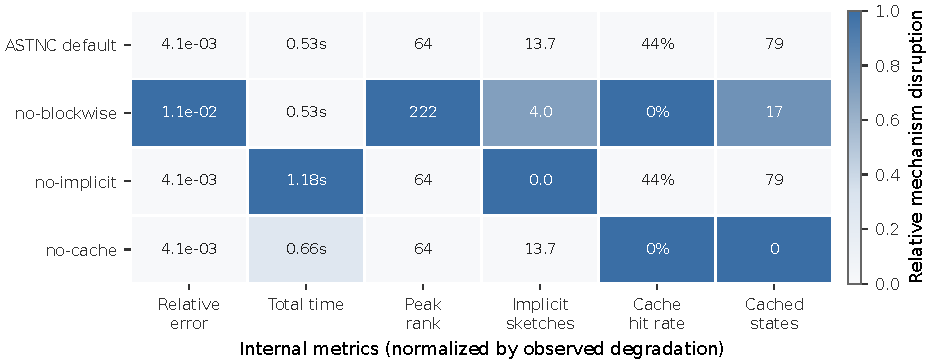
\includegraphics[width=\columnwidth]{figures_strengthened/fig_mechanism_fingerprint_grid.pdf}
\caption{Grid $3\times 3$ 上的机制指纹图。按指标归一化后，不同变体的主要退化方向变得更清晰：no-blockwise 主要抬高误差与峰值秩，no-implicit 主要恶化运行时间，no-cache 则主要击穿复用相关统计。}
\label{fig:mechanism_fingerprint_grid}
\end{figure}

\paragraph{输出分块作为设计空间。}
为了进一步理解默认配置为何选择“沿前两个输出轴、按单索引块逐块生成”的设置，我们在 Grid $3\times 3$ 上做了局部 blockwise 扫描。
\Cref{fig:blockwise_operating_points_grid} 以设计空间的方式展示了这些结果：主图聚焦 practical operating region，而 near-exact 的设置被单独放入 inset，从而避免极小误差点把整张图的误差轴压扁。
在这样的视图下，正文默认配置的角色更清楚了：它并不是误差最低、也不是时间最短，而是在当前候选项中提供了更均衡的工作点。
因此，默认设置并不是任意选取，而是在误差、时间、峰值秩与复用行为之间做出的平衡。

\begin{figure}[t]
\centering
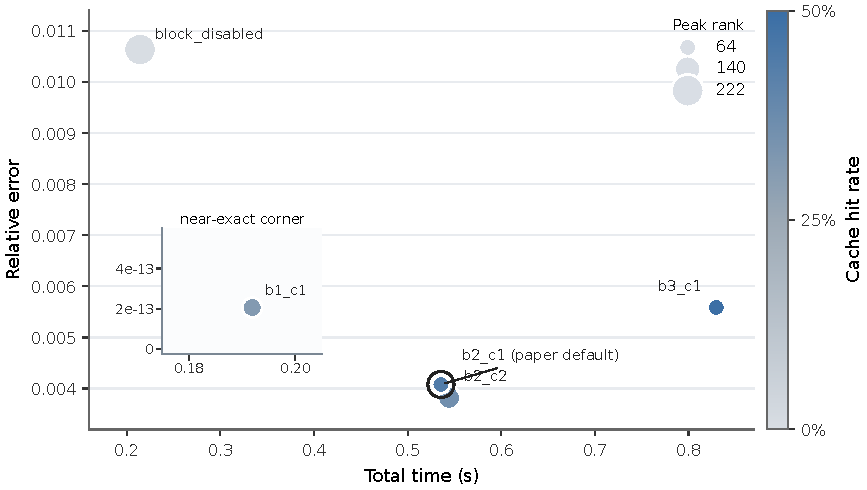
\includegraphics[width=\columnwidth]{figures_strengthened/fig_blockwise_operating_points_grid.pdf}
\caption{Grid $3\times 3$ 上的 blockwise 设计空间。主图聚焦 practical operating region，点面积编码 peak rank、颜色编码 cache hit rate；inset 单独展示 near-exact 设置，从而使正文默认配置能以“平衡点”而非“被压扁的中间点”被读出。}
\label{fig:blockwise_operating_points_grid}
\end{figure}